\section{The Higgs Mechanism and Electroweak Symmetry Breaking}
\label{sec:higgs_description}

The missing mass-terms for the fields in \SML~are provided by the
Brout-Englert-Higgs (BEH) mechanism~\cite{Englert:1964et,Higgs:1964ia,Higgs:1964pj}.
Before describing the specifics of the BEH mechanism, we should first describe the problem
of why \SML~doesn't support general mass terms for any of the fields in the first place.
That is, for example, why can't a fermion term like $m \bar{f} f$ exist in \SML?

Adding mass terms to \SML~for the fermions explicitly breaks the underlying \SUtwo~
gauge symmetry. This can be understood if we recognize the experimentally supported
fact that the left-handed fermions appear as \SUtwo~doublets and that the
right-handed fermions as singlets,
\begin{align}
	m\bar{f}f &= m \bar{f}(P_L + P_R)f \notag \\
				   &= m \bar{f} P_L P_L f + m \bar{f} P_R P_R f  	\label{eq:bad_fermion_mass_term}\\
				   &= m \left( \bar{f}_R f_L + \bar{f}_L f_R \right), \notag
,
\end{align}
where we have used identity relations of the projection operators $P_L$ and $P_R$ and the fact that $\bar{f}P_L = \bar{f}_R$ (and vice-versa). The last line of Eqn.~\ref{eq:bad_fermion_mass_term} involve terms
mixing \SUtwo~doublets with \SUtwo~singlets. Such a term is therefore not allowed if we wish to keep the \SUtwo~gauge symmetry intact.

Mass terms for the gauge bosons, of the form $m B_{\mu} B^{\mu}$, also do not work. For the Abelian \Uone~symmetry, for example, gauge invariance implies invariance of \SML~under transformations
of the form $B_{\mu}^{\prime} \rightarrow B_{\mu} - \partial_{\mu}\chi /g$. Such a mass term for
the gauge bosons is clearly not invariant under such a transformation. Even forgoing this fact,
adding such a term would quickly lead to non-renormalisable divergences appearing in the theory,
due to the longitudinal field components that appear in massive field propagators, rendering \SML~meaningless.

The BEH mechanism provides a way out of this problem. It refers to the introduction of a
spin-0 field, theHiggs field (Table \ref{tab:sm_content}), to the SM along with its corresponding interaction
terms to \SML: the last three terms of Eqn.~\ref{eq:sm_lagrangian}. These terms make up
what is referred to as the Higgs potential which can be expressed as (ignoring the
kinetic terms proportional to $\mathit{D}_{\mu}$),
\begin{align}
	V(\phi) = - \mu^2 \phi^2 - \lambda \phi^4
	\label{eq:higgs_potential}
\end{align}
The Higgs field is an \SUtwo~doublet and it can be seen that the interactions
described by Eqn.~\ref{eq:higgs_potential} respect \SUtwo~gauge symmetry.
If $\mu^2>0$, nothing all too interesting occurs and Eqn.~\ref{eq:higgs_potential} describes
a self-interacting, complex scalar field. If we take $\mu^2<0$, however, then the classical
potential described by Eqn.~\ref{eq:higgs_potential} has non-zero minima located at
$\phi = \pm v$ with $v = \sqrt{-\mu^2 / \lambda}$.
This is illustrated in Fig.~\ref{fig:higgs_ewsb}. We see that the stable equilibrium point
of the Higgs potential, the \textit{Higgs vacuum expectatin value} (vev), is not at $\phi = 0$
but at $v$,
\begin{align}
	\phi_0 = \frac{1}{\sqrt{2}} \left( \begin{matrix} 0 \\ v \end{matrix} \right)
	\label{eq:higgs_vev}
\end{align}
The choice of Eqn.~\ref{eq:higgs_vev} to represent the Higgs vacuum is motivated by
the requirement that the vacuum not be electrically charged --- a fact motivated very much
by experiment and everyday experience --- so the up-type \SUtwo~component of the Higgs field, $\phi^+$ (Table \ref{tab:sm_content}), is chosen to be zero for $\phi_0$. The choice of an
electrically neutral vacuum sets the rest of the \SUewk~structure of the complex Higgs field
since, by the Gell-Mann-Nishijima relation (Eqn.~\ref{eq:gell_mann_nishijima}) and charge
conservation,
a  neutral \SUewk~field should have down-type \SUtwo~quantum numbers and \Uone~hypercharge
$Y=1$,
\begin{align}
	Q = T_3 + \frac{1}{2}Y \rightarrow Q_{\phi_0} = -\frac{1}{2} + \frac{1}{2} \times 1 = 0.
\end{align}

Note that Eqn.~\ref{eq:higgs_vev} states that only one component of the Higgs \SUtwo~doublet
attains a non-zero vev. This clearly means that the \SUtwo~gauge symmetry is not respected
by the choice of $\mu^2 < 0$ and that the electroweak \SUewk~symmetry is
\textit{spontaneously broken}.\footnote{A symmetry of a Lagrangian is said to be
	`spontaneously' broken if the Lagrangian of the underlying theory
	respects the symmetry but it gets broken through dynamical means or if the lowest-energy
	state (vacuum) does not respect the symmetry.
} The Higgs field
acquiring a non-zero vev is then referred to as the \textit{electroweak symmetry breaking} (EWSB) of the SM.

To further examine the physical consequences of EWSB,
we perturb the Higgs field about the its minimum value of $v$,
\begin{align}
	\phi(x) \propto \left( \begin{matrix} 0 \\ \frac{1}{2}(v + h(x)) \end{matrix} \right),
	\label{eq:higgs_perturb}
\end{align}
where $h(x)$ correspond to excitations of the Higgs field that represent the physically observable
Higgs boson. If we plug Eqn.~\ref{eq:higgs_vev} into the $\mathit{D}_{\mu}\phi$ terms
of Eqn.~\ref{eq:sm_lagrangian}, one eventually works through the algebra and obtains,
\begin{align}
	\lvert\mathit{D}_{\mu} \phi(x)\rvert^2 = \frac{1}{8} v^2 g_2^2 \left[ \left( W^1_{\mu} \right)^2 +\left( W^2_{\mu} \right)^2 \right] 
		+ \frac{1}{8} v^2 \left( g_1 B_{\mu} - g_2 W_{\mu}^3 \right)^2.
	\label{eq:higgs_gauge_expand} 
\end{align}
{\color{red}{mention gauge-boson-higgs interactions / diagrams?}}
Using the field re-definitions for the $W_{\mu}$, $A_{\mu}$ and $Z_{\mu}$ introduced in Section~\ref{sec:ewk_description}, we see that this can be re-written as (modulo factors of 2),
\begin{align}
	\lvert\mathit{D}_{\mu} \phi(x)\rvert^2 \propto \left(\frac{1}{2} v g_2 \right)^2 W_{\mu}^+ W^{-\,\mu} + \left( \frac{1}{2}v \sqrt{g_1^2 + g_2^2} \right)^2 Z_{\mu} Z^{\mu} + (0)^2 A_{\mu} A^{\mu},
	\label{eq:higgs_gauge_masses}
\end{align}
which provide, clearly, mass terms for the electroweak gauge bosons:
\begin{align}
	M_W = \frac{1}{2}v g_2, \hspace{1cm} M_Z = \frac{1}{2}v\sqrt{g_1^2 + g_2^2}, \hspace{1cm} M_A = 0.
	\label{eq:gauge_boson_masses}
\end{align}

\begin{figure}[!htb]
	\begin{center}
		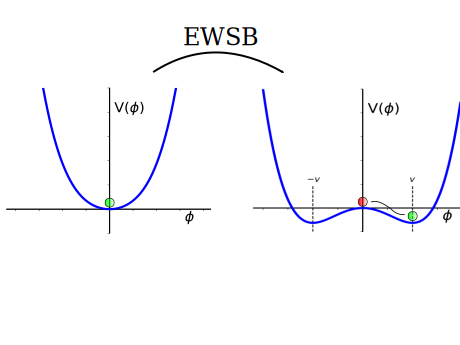
\includegraphics[width=\textwidth]{figures/chapter1/higgs_potential_trans}
		\caption{Illustration of electroweak symmetry breaking (EWSB).
			\textit{Left}: Higgs potential with $\mu^2>0$ with stable equilibrium at $\phi=0$.
			\textit{Right}: With $\mu^2<0$, $\phi=0$ is no longer
			a stable equilibrium and the Higgs attains a non-zero vacuum
			expectation value at $\pm v$ --- breaking the \SUewk~gauge symmetry of the electroweak
			sector of the SM.
		}
	\label{fig:higgs_ewsb}
	\end{center}
\end{figure}

The masses of the fermions can be obtained by adding the interaction terms such as the following:
\begin{align}
	\mathcal{L}_{f-h} = g_e \left( \bar{L} \phi e^-_R + \phi^{\dagger} \overline{e^-}_R L\right).
	\label{eq:higgs_fermion_int}
\end{align}
Since both $L$ and $\phi$ are \SUtwo~doublets, adding the right-handed \SUtwo~singlet terms
do not spoil the \SUtwo~symmetry. We can require EWSB and insert Eqn.~\ref{eq:higgs_perturb} 
into Eqn.~\ref{eq:higgs_fermion_int} resulting in,
\begin{align}
	\mathcal{L}_{f-h} = \frac{1}{\sqrt{2}} y_f v \left( \overline{f^-_L} f^-_R + \overline{f^-_R} f^-_L \right)
	+ \frac{1}{\sqrt{2}} \left( \overline{f^-_L}f^-_R + \overline{f^-_R} f^-_L \right) h,
	\label{eq:higgs_fermion_ewsb}
\end{align}
from which we can read off the fermion mass terms as,
\begin{align}
	m_f = y_f \frac{v}{\sqrt{2}},
	\label{eq:fermion_mass_term}
\end{align}
where the $y_f$ are referred to as the fermion \textit{Yukawa couplings}, and are free parameters
of the SM that need to be measured. Given this form for the masses of the fermions,
we can see from
the second term of Eqn.~\ref{eq:higgs_fermion_ewsb}
that the coupling of the Higgs to a given fermion species is directly related to the 
fermion's mass. To make this obvious, we re-write Eqn.~\ref{eq:higgs_fermion_ewsb} as,
\begin{align}
	\mathcal{L}_{f-h} = \underbrace{m_f \bar{f} f}_\text{$f$ mass term} + \underbrace{\frac{m_f}{v} \bar{f}f h}_\text{$f-h$ coupling}.
	\label{eq:higgs_fermion_coupling}
\end{align}




